\documentclass[10pt,twocolumn,letterpaper]{article}
\usepackage[pagenumbers]{cvpr}
\usepackage{graphicx,amsmath,amssymb,booktabs,multirow,xcolor}
\usepackage[font=small,skip=3pt]{caption}
\definecolor{cvprblue}{rgb}{0.21,0.49,0.74}
\usepackage[breaklinks,colorlinks,allcolors=cvprblue]{hyperref}
\setlength{\textfloatsep}{8pt plus 2pt minus 2pt}
\setlength{\floatsep}{6pt plus 2pt minus 2pt}
\setlength{\dbltextfloatsep}{8pt plus 2pt minus 2pt}
\setlength{\tabcolsep}{4pt}
\newcommand{\pct}[1]{#1\%}
\def\confName{CVPR}
\def\confYear{2026}

\title{Bagging, Boosting and Measured Bias--Variance on Olivetti Faces}
\author{Sourabh Singh \quad Roll no.\ M25CPS009\\
Indian Institute of Technology, Jodhpur\\
{\small Machine Learning, Assignment 2}\\
{\small Code: \url{\REPOURL} \quad Commit: \texttt{\COMMIT}}}
\newcommand{\REPOURL}{https://github.com/Sourabh16/Machine-Learning-Assignment2-Bagging-Boosting}
\newcommand{\COMMIT}{483f9f0}


\begin{document}
\maketitle

\begin{abstract}
I compare a single decision tree, bagging and multiclass SAMME boosting for
face identification on raw Olivetti pixels. Bagging and boosting are my own
implementations on top of scikit-learn's \texttt{DecisionTreeClassifier}. On
clean test faces the tree gets \pct{55.0}, bagging (200 trees) \pct{81.3} and
boosting (depth 4, 100 rounds) \pct{46.3}; with the centre of the face masked
these drop to \pct{23.8}, \pct{67.5} and \pct{35.0}. Over 30 resampled
training sets bagging removes about 96\% of the tree's variance, while boosting
has the lowest variance but the highest bias and worst accuracy.
\end{abstract}

%=====================================================================
\section{Setup}
\label{sec:setup}
\textbf{Data and split.} The seed is the digits of my roll number,
\texttt{default\_rng(25009)}. For each of the 40 people I shuffle the ten
images and keep 6 for training, 2 for validation and 2 for test (240/80/80).
The split is saved in \texttt{splits/} and reused by every script. I use the
4096 raw pixels with no PCA. The masked test set is a copy of the test images
with rows and columns 24--39 set to zero (\cref{fig:mask}); training only ever
uses clean images.

\textbf{Implementation.} Bagging and SAMME are in \texttt{src/ensembles.py}.
Bagging draws a bootstrap of 240 images and a tie-breaking seed for each tree
in turn, so the first $B$ trees of the 200-tree model are exactly the $B$-tree
model and every $B$ can be read from one fit (refitting at 25/50/100 trees in
Q2(c) gives the same numbers). It predicts by majority vote, and its
confidence is the winning vote fraction.

\textbf{Selection.} Every choice uses clean validation accuracy only, with ties
going to the simpler model. Test accuracy was only looked at after freezing.

\begin{figure}[t]
\centering
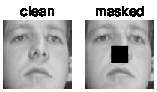
\includegraphics[width=0.36\linewidth]{../figures/mask_example.pdf}
\caption{A test face and its masked copy (rows/cols 24--39 set to 0).}
\label{fig:mask}
\end{figure}

%=====================================================================
\section{Q1: Single tree and bagging}
\subsection{(a) Single-tree baseline}
\Cref{tab:tree} shows the grid. For every capped depth the three leaf sizes
give the same tree, since no leaf is small enough for the limit to matter. The
best validation accuracy (\pct{53.8}) is for \texttt{max\_depth=None},
\texttt{min\_samples\_leaf=4}, which I froze.

\begin{table}[t]
\centering\small
\begin{tabular}{lcccccc}
\toprule
max\_depth / leaf & train & val & test & leaves & per leaf & single\\
\midrule
2 / any        & 7.5  & 7.5  & 7.5  & 3  & 80.0 & 0\\
4 / any        & 12.5 & 11.3 & 11.3 & 5  & 48.0 & 0\\
8 / any        & 22.5 & 18.8 & 21.3 & 9  & 26.7 & 0\\
16 / any       & 42.5 & 31.3 & 32.5 & 17 & 14.1 & 0\\
None / 1       & 100  & 48.8 & 55.0 & 46 & 5.2  & 0.13\\
None / 2       & 97.5 & 48.8 & 53.8 & 46 & 5.2  & 0\\
\textbf{None / 4} & \textbf{96.3} & \textbf{53.8} & \textbf{55.0} & \textbf{40} & \textbf{6.0} & \textbf{0}\\
\bottomrule
\end{tabular}
\caption{Single-tree grid (accuracy in \%). ``per leaf'' is the mean number of
training images per leaf and ``single'' the fraction of leaves holding exactly
one training image. The frozen tree (bold) has realised depth 36.}
\label{tab:tree}
\end{table}

\textbf{What changes with depth.} The trees are very lopsided: a tree capped at
depth $d$ has exactly $d+1$ leaves (\cref{fig:depth}). Each split peels a few
faces off and leaves one big mixed node, because one pixel threshold can
separate one person from the rest but not 20 people from 20. So a depth-16 tree
can name at most 17 of the 40 people, which is why training accuracy is only
\pct{42.5} and accuracy grows almost linearly with depth. Only unbounded trees
(36--37 levels, 40--46 leaves) fit the data. With leaf size 1, 13\% of leaves
hold one image and training accuracy is \pct{100}; leaf size 4 gives 40 leaves
of about six images, roughly one per person, losing 3.8 training points but
gaining 5 on validation. Deeper trees reduce bias, but at full depth they start
memorising single images.

\begin{figure}[t]
\centering
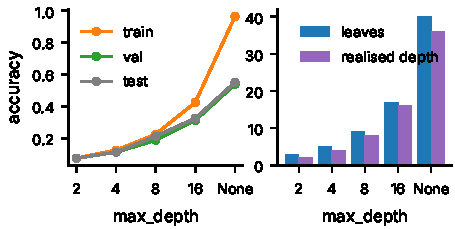
\includegraphics[width=\linewidth]{../figures/q1a_depth.pdf}
\caption{Left: accuracy against \texttt{max\_depth} (\texttt{min\_samples\_leaf=4}).
Right: leaves and realised depth. Leaves $=$ depth$+1$ for every capped tree.}
\label{fig:depth}
\end{figure}

\subsection{(b) Bagging from scratch}
\Cref{tab:bag} gives the results. A bootstrap of size $n$ should contain
$n[1-(1-1/n)^n] = 151.89$ distinct images ($0.633n$, close to $1-e^{-1}$). Over
the 200 bootstraps I measured $151.6 \pm 4.7$ (139--167), which matches.
Training accuracy reaches \pct{100} by $B=50$, and test accuracy goes from
\pct{40.0} for one bagged tree (it sees only about 152 distinct images) to
\pct{81.3} at $B=200$.

\begin{table}[t]
\centering\small
\begin{tabular}{rcccccccc}
\toprule
$B$ & train & val & test & distinct & OOB & dis. & margin\\
\midrule
1   & 67.9 & 40.0 & 40.0 & 154.0 & 31.4$^\dagger$ & -- & 1.00\\
5   & 90.4 & 55.0 & 46.3 & 151.0 & 29.9$^\dagger$ & .755 & .270\\
10  & 98.8 & 72.5 & 58.8 & 153.4 & 39.8$^\dagger$ & .778 & .258\\
25  & 99.6 & 70.0 & 71.3 & 151.9 & 55.4 & .799 & .241\\
50  & 100  & 80.0 & 72.5 & 151.8 & 68.3 & .790 & .255\\
100 & 100  & 78.8 & 78.8 & 151.7 & 75.4 & .793 & .261\\
\textbf{200} & 100 & \textbf{81.3} & \textbf{81.3} & 151.6 & 77.1 & .801 & .250\\
\bottomrule
\end{tabular}
\caption{Bagging the frozen tree. ``distinct'' is the mean number of distinct
training images per bootstrap (theory 151.89). OOB, mean pairwise
disagreement (``dis.'') and mean vote margin use the first $B$ trees; dis.\
and margin are measured on the validation set. $^\dagger$Only 36\%, 89\% and
98\% of training images have at least one out-of-bag tree at $B=1,5,10$.}
\label{tab:bag}
\end{table}

\subsection{(c) OOB accuracy, disagreement and vote margin}
\Cref{fig:bagc} shows the three quantities against $B$. Validation accuracy is
highest at $B=200$ (\pct{81.3}, against \pct{80.0} at 50 and \pct{78.8} at 100),
so the final model uses 200 trees.

The three curves do not tell the same story. \emph{OOB accuracy} tracks
validation accuracy and is still rising at 200 (\pct{75.4}$\to$\pct{77.1}). It
sits a little lower because each image is out-of-bag for only about $0.37B$
trees, and below $B=25$ it does not cover every image. \emph{Disagreement} is
flat at about 0.80 (two trees disagree on four of five faces), since it is a
property of the base tree rather than of $B$. The \emph{mean margin} falls from
1 to about 0.25 by $B=5$ and then stays put.

So adding trees does not make each face more confidently classified; it makes
the plurality more reliable, since the noise in which class wins shrinks like
$1/\sqrt{B}$. Disagreement and margin describe the trees, which the tree
setting fixes; OOB and validation accuracy show how far the averaging has
converged.

\begin{figure*}[t]
\centering
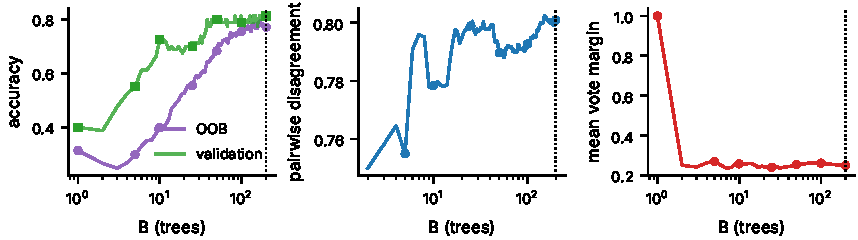
\includegraphics[width=0.85\linewidth]{../figures/q1c_bagging.pdf}
\caption{Bagging diagnostics against $B$ (log scale). Lines are evaluated at
every $B$, markers at the required sizes, and the dotted line is the selected
$B=200$. Disagreement and margin are on the validation set.}
\label{fig:bagc}
\end{figure*}

\subsection{(d) Tree versus bagging, clean and masked}
\begin{table}[t]
\centering\small
\begin{tabular}{llcccc}
\toprule
& & \multicolumn{2}{c}{clean} & \multicolumn{2}{c}{masked}\\
& & acc & conf & acc & conf\\
\midrule
\multicolumn{2}{l}{Tree (leaf probability)} & 55.0 & .971 & 23.8 & 1.000\\
\multicolumn{2}{l}{Bagging, $B{=}200$ (win.\ vote)} & 81.3 & .356 & 67.5 & .258\\
\midrule
\multicolumn{2}{l}{Bagging conf.\ if correct / wrong} & \multicolumn{2}{c}{.390 / .212} & \multicolumn{2}{c}{.301 / .167}\\
\multicolumn{2}{l}{Bagging disagreement (test)} & \multicolumn{2}{c}{.810} & \multicolumn{2}{c}{.881}\\
\bottomrule
\end{tabular}
\caption{Frozen tree and final bagged model on the two test sets.}
\label{tab:q1d}
\end{table}

\Cref{tab:q1d} compares the two. The tree is about as confident when wrong as
when right (0.96 vs 0.98), so its confidence is useless. Bagging's winning vote
is lower but meaningful (0.39 when right, 0.21 when wrong). Masking wrecks the
tree: 54 of the 80 masked faces fall into a single leaf (identity~35), masked
faces reach only 12 leaves instead of 37, and accuracy drops to \pct{23.8} at
confidence 1.0. Bagging loses 14 points, and its disagreement rises from 0.81
to 0.88, so it at least shows that it is less sure.

On clean faces bagging fixes 23 of the tree's mistakes, adds 2, and 13 are
wrong for both (\cref{fig:cases}). \textbf{Fixed:} the tree calls face 338
(identity 33) ``23'' with confidence 1.0, but only 7 of 200 trees agree and 119
vote 33; face 175 (identity 17) is ``3'' for the tree but gets 112 votes for 17.
These mistakes came from one particular path of thresholds, which other
bootstrap trees do not repeat, so they average out: \emph{variance} errors.
\textbf{Both wrong:} face 234 (identity 23) gets 72 votes for 13 and only 6 for
the truth, and face 251 (identity 25) gets 67 votes for 37 against 38. Here the
trees agree on the wrong person, and the other image of identity 25 also goes
to 37, so these two people simply look alike to the trees. Averaging cannot
move the average prediction, so these \emph{bias} errors remain.

\begin{figure}[t]
\centering
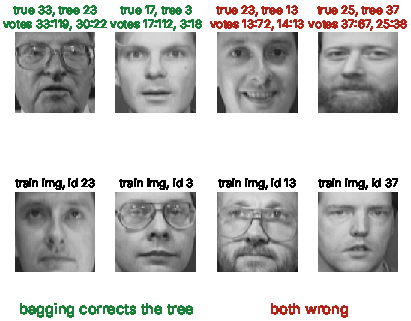
\includegraphics[width=\linewidth]{../figures/q1d_cases.pdf}
\caption{Top: test faces with the tree prediction and the top two bagging vote
counts (out of 200). Bottom: a training image of the identity that was wrongly
predicted (tree's guess for the corrected cases, bagging's for the failures).}
\label{fig:cases}
\end{figure}

%=====================================================================
\section{Q2: Multiclass SAMME boosting}
My SAMME uses $\alpha_t=\log\frac{1-\epsilon_t}{\epsilon_t}+\log(K-1)$,
multiplies the weights of misclassified images by $e^{\alpha_t}$ and
renormalises, predicts with $S_k(x)=\sum_t\alpha_t\mathbb 1[h_t(x)=k]$ and uses
$q_k=S_k/\sum_t\alpha_t$ as confidence. A learner with
$\epsilon_t\ge1-1/K$ would get $\alpha_t\le0$, so I reject it, keep the weights,
and refit with a new seed, stopping after five rejections in a row. A perfect
learner would get infinite $\alpha$, so $\epsilon$ is clipped at $10^{-10}$ and
boosting stops. Neither case occurred: after round 5 the largest error was
0.74, far below 0.975.

\subsection{(a) One logged round on a toy problem}
\begin{table}[t]
\centering\small
\begin{tabular}{ccccccc}
\toprule
$i$ & $x_i$ & $y_i$ & $w_i^{(0)}$ & $h_1(x_i)$ & miss & $w_i^{(1)}$\\
\midrule
0--2 & (1,1),(1.5,2),(2,1.2) & 0 & 1/9 & 0 & 0 & 0.0556\\
3--4 & (4,4),(4.5,3.5)       & 1 & 1/9 & 1 & 0 & 0.0556\\
5    & (2.2,1.6)             & 1 & 1/9 & 1 & 0 & 0.0556\\
6--7 & (7,1),(6.5,2)         & 2 & 1/9 & 1 & 1 & 0.2222\\
8    & (4.2,3.8)             & 2 & 1/9 & 1 & 1 & 0.2222\\
\bottomrule
\end{tabular}
\caption{One SAMME round on 9 points and 3 classes with a depth-1 stump
($x_1\le2.1\Rightarrow0$, else 1). $\epsilon_1=3/9$,
$\alpha_1=\log2+\log2=1.386$; misclassified weights are multiplied by
$e^{\alpha_1}=4$ before renormalising.}
\label{tab:toy}
\end{table}

\Cref{tab:toy} is the round-one log from the same class used on the faces,
checked against a hand calculation. A stump can name only two of the three
classes, so all of class 2 is wrong, but $\epsilon=1/3$ is still below the
random level $2/3$, so $\alpha_1>0$.

One useful fact falls out of the update: the misclassified images always end
up with exactly $(K-1)/K$ of the total weight, whatever $\epsilon_t$ is (here
$2/3$). On the faces that is $39/40$, so the images a learner got right keep
only 2.5\% of the weight between them.

\subsection{(b) Depth and number of rounds}
\begin{table}[t]
\centering\small
\begin{tabular}{lcccc}
\toprule
depth $\backslash$ rounds & 10 & 25 & 50 & 100\\
\midrule
1 & 3.8 & 7.5 & 8.8 & 10.0\\
2 & 3.8 & 11.3 & 15.0 & 22.5\\
3 & 16.3 & 18.8 & 26.3 & 33.8\\
4 & 26.3 & 28.8 & 36.3 & \textbf{50.0}\\
\bottomrule
\end{tabular}
\caption{Clean validation accuracy (\%) of SAMME. The selected model (depth 4,
100 rounds) has \pct{99.6} train and \pct{46.3} test accuracy.}
\label{tab:boostgrid}
\end{table}

\Cref{tab:boostgrid} shows the grid; depth 4 with 100 rounds is selected.
Accuracy rises along both axes because the learners really are weak: a
depth-$d$ tree can name at most $2^d$ people (2 for a stump, 16 at depth 4), and
stumps reach only \pct{10}. At depth 4 the validation curve is still rising at
100 rounds, so the grid is the limit.

In \cref{fig:boostdiag}, the weighted error starts at 0.85 and settles around
0.66: far below 0.975 but large, since a 16-leaf tree must miss at least 24
people. $\alpha$ stays near 3.0. Weights concentrate fast: the largest goes from
0.0042 to 0.054 (13 times uniform), and the ten heaviest images (4\% of the
data) hold 14--40\% of the weight after round 20. The saw-tooth pattern is the
$(K-1)/K$ rule: heavy faces that a learner gets right lose most of their weight
at once, then regain it when later learners miss them.

\begin{figure*}[t]
\centering
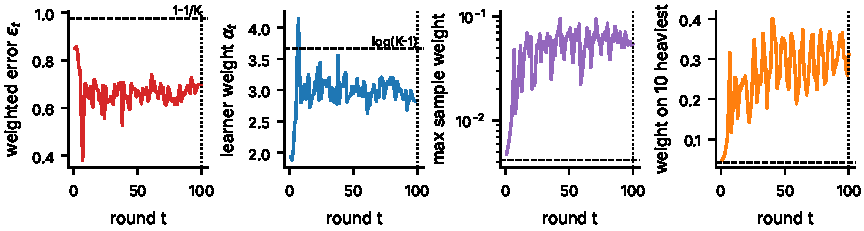
\includegraphics[width=0.92\linewidth]{../figures/q2b_diagnostics.pdf}
\caption{Selected SAMME run (depth 4): weighted training error (dashed: random
level $1-1/K$), learner weight (dashed: $\log(K-1)$, \ie $\epsilon=0.5$),
largest sample weight (log scale, dashed: uniform $1/240$) and total weight of
the 10 heaviest training images (dashed: uniform 10/240).}
\label{fig:boostdiag}
\end{figure*}

\subsection{(c) Boosting versus bagging at equal size}
\begin{table}[t]
\centering\small
\begin{tabular}{llccccc}
\toprule
& $M$ & train & val & test & time (s)\\
\midrule
\multirow{3}{*}{SAMME (depth 4)} & 25 & 60.8 & 28.8 & 30.0 & 5.7\\
& 50 & 87.5 & 36.3 & 42.5 & 11.0\\
& 100 & 99.6 & 50.0 & 46.3 & 22.5\\
\midrule
\multirow{3}{*}{Bagging (full trees)} & 25 & 99.6 & 70.0 & 71.3 & 17.5\\
& 50 & 100 & 80.0 & 72.5 & 34.4\\
& 100 & 100 & 78.8 & 78.8 & 69.5\\
\bottomrule
\end{tabular}
\caption{Equal numbers of learners, each model refitted from scratch on one
core. Bagging's numbers match \cref{tab:bag}, which confirms the prefix
property.}
\label{tab:cmp}
\end{table}

\Cref{tab:cmp} compares them at equal size. Bagging is 25--40 points better
everywhere, while boosting is about three times faster per learner (0.22\,s vs
0.7\,s per tree). Boosting reaches \pct{99.6} on training data but only \pct{50}
on validation, with very small margins (0.026 against 0.23 for bagging).

\textbf{A heavily weighted face.} Training image 87 (identity 8) ends with the
largest weight, 0.054 (\cref{fig:heavy}). Only 12 of the 100 learners get it
right; it is most often called 2, a similar-looking person. Each correct
learner cuts its weight by more than ten times, but the next 16-leaf tree
usually has no room for identity 8, gets it wrong, and multiplies its relative
weight by $e^{\alpha}\approx20$. So boosting keeps coming back to it, not
because the label is wrong but because no single weak learner can hold it. The
full ensemble does classify it correctly in the end.

\begin{figure}[t]
\centering
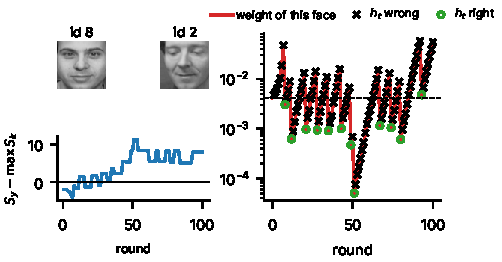
\includegraphics[width=\linewidth]{../figures/q2c_heavy.pdf}
\caption{Training image 87 (identity 8) and a training image of identity 2,
its most frequent confusion. Right: its sample weight per round (log scale)
with the correctness of $h_t$. Bottom left: its ensemble margin
$S_y-\max_{k\ne y}S_k$ over rounds.}
\label{fig:heavy}
\end{figure}

\subsection{(d) Robustness to the missing region}
\begin{table}[t]
\centering\small
\begin{tabular}{lcccc}
\toprule
& \multicolumn{2}{c}{clean} & \multicolumn{2}{c}{masked}\\
& acc & conf & acc & conf\\
\midrule
Single tree (leaf prob.) & 55.0 & .971 & 23.8 & 1.000\\
Bagging, 200 (win.\ vote) & \textbf{81.3} & .356 & \textbf{67.5} & .258\\
SAMME, d4/100 (max $q_k$) & 46.3 & .114 & 35.0 & .104\\
\bottomrule
\end{tabular}
\caption{Frozen models on clean and masked test faces. Confidence is the mean
winning probability or vote. Accuracy drops: tree $-31.3$, bagging $-13.8$,
boosting $-11.3$ points.}
\label{tab:q2d}
\end{table}

\Cref{tab:q2d} shows all three models. Boosting loses the fewest points
(11.3) mostly because it started low. Under masking, 41 of the 80 faces are
predicted as identity~30. Boosting has a similar ``sink'' even on clean faces:
identity 2 gets 9.4\% of the total $\alpha$ on an average test face (four
times its fair share), because weak trees often use it to label a big
catch-all leaf, and 35 clean faces end up as 2. A zero block is darker than any
real face, so many learners send masked faces the same way and identity 30
collects the votes.

\textbf{Example: test face 17 (identity 1).} Bagging is right on both versions
(125 votes clean, 79 masked, best rival 19). Boosting is right when clean but
says 30 when masked ($q_1$: $0.117\to0.077$, $q_{30}=0.098$). \emph{Bagging:}
masking changes 46\% of the trees' votes and disagreement on this face rises
from 0.61 to 0.82, but the changed votes scatter over several people and
identity 1 started far ahead, so it still wins. \emph{Boosting:} learners
holding 29\% of the $\alpha$ change their vote, four of them away from identity
1 and none towards it. The real problem is the clean margin, only 0.01 over
identity 2. Because the $(K-1)/K$ rule keeps moving the weight to whatever the
last learner missed, each identity is backed by only a small slice of the
$\alpha$ mass, and the learners also lean on central pixels slightly more than
chance (8.1\% of $\alpha$-weighted splits in a block that is 6.25\% of the
image). A few flipped learners are enough. Bagging's large plurality absorbs
the extra disagreement; boosting's thin, weight-driven margin does not.

%=====================================================================
\section{Q3: Bias and variance as measured quantities}
I keep the clean test set fixed and build 30 training sets, each drawing 6
faces with replacement from every person's 6 training faces (about 4 distinct
faces per person). The three selected models are refitted on each set without
retuning. The class vector is the leaf distribution (tree), the vote fractions
(bagging) or $q$ (boosting), and bias$^2$+variance is the mean squared distance
to the one-hot target.

\subsection{(a) Selected models}
\begin{table}[t]
\centering\small
\begin{tabular}{lcccc}
\toprule
& bias$^2$ & variance & sum & test acc.\ (30 refits)\\
\midrule
Tree     & .475 & .670 & 1.145 & $42.8 \pm 5.0$\\
Bagging  & .558 & .020 & .578  & $71.7 \pm 4.3$\\
Boosting & .885 & .018 & .903  & $33.9 \pm 7.3$\\
\bottomrule
\end{tabular}
\caption{Measured bias$^2$ and variance on the clean test set, and mean $\pm$
standard deviation of test accuracy across the 30 refits.}
\label{tab:q3a}
\end{table}

\Cref{tab:q3a} gives the results. Accuracies are lower than for the frozen
models because each set has fewer distinct images, but the ranking holds. The
tree has by far the largest variance (0.67), and bagging removes 97\% of it.
Bagging's bias$^2$ is \emph{higher} than the tree's (0.558 vs 0.475), which
surprised me at first. The reason is that bias is measured on vectors: bagging's
votes are spread out (winning share about 0.36), so even its average vector is
far from one-hot. Taking the argmax of the average vector instead, bagging is
right on 85\% of faces and the tree on 71\%. The total error (0.58 vs 1.15)
matches the accuracy ranking. Boosting has the lowest variance but the highest
bias and the lowest, least stable accuracy ($33.9\pm7.3$).

\subsection{(b) Effect of depth}
\begin{table*}[t]
\centering\small
\begin{tabular}{lccccccccccc}
\toprule
& \multicolumn{2}{c}{single tree} & \multicolumn{2}{c}{bagging (100 trees)} & var.\ removed & \multicolumn{3}{c}{test accuracy (\%)} & & & \\
\cmidrule(lr){2-3}\cmidrule(lr){4-5}\cmidrule(lr){7-9}
max\_depth / leaf & bias$^2$ & var & bias$^2$ & var & abs.\ (frac.) & tree & bag & gain & disagr. & leaves & per leaf\\
\midrule
2 / 4  & .934 & .041 & .932 & .011 & .030 (73\%) & 5.1  & 15.5 & +10.4 & .961 & 3.0  & 80.0\\
\textbf{4 / 4 (shallow)}  & .894 & .073 & .893 & .012 & .061 (83\%) & 8.8  & 28.5 & +19.7 & .949 & 5.2  & 46.2\\
8 / 4  & .809 & .146 & .817 & .016 & .131 (89\%) & 15.0 & 43.3 & +28.3 & .928 & 9.5  & 25.4\\
16 / 4 & .689 & .271 & .690 & .020 & .251 (93\%) & 25.2 & 59.8 & \textbf{+34.6} & .894 & 17.9 & 13.4\\
\textbf{None / 4 (selected)} & .475 & .670 & .558 & .024 & .646 (96\%) & 42.8 & 70.5 & +27.8 & .834 & 40.0 & 6.0\\
\textbf{None / 1 (deepest)}  & .475 & .670 & .537 & .024 & .646 (96\%) & 42.8 & 73.6 & +30.8 & .824 & 40.0 & 6.0\\
\bottomrule
\end{tabular}
\caption{Depth study over the 30 resampled training sets (means). ``disagr.''
is the mean pairwise disagreement of the bagged trees on the test set; leaves
and images per leaf are for the single tree. With
\texttt{min\_samples\_leaf=1} the bagged trees have 46.5 leaves on average and
13.4\% of their leaves hold one image; with 4 they have 39.2 leaves and none.}
\label{tab:depth}
\end{table*}

The selected tree is already unbounded, so for the ``much deeper'' tree I
remove the leaf-size floor (leaf size 1). Depth 4 is the shallow tree, and I
also ran depths 2, 8 and 16 for part (c) (\cref{tab:depth}, \cref{fig:q3}).

Going deeper halves the tree's bias$^2$ (0.93 to 0.48) while its variance
grows about 16 times (0.04 to 0.67). Shallow trees have low variance only
because, with 3--5 leaves, they predict almost the same thing every time.

Bagging removes 73\% of the variance at depth 2, 83\% at depth 4, 93\% at
depth 16 and 96\% for unbounded trees (0.03, 0.06, 0.25 and 0.65 in absolute
terms). Its own variance stays between 0.011 and 0.024 at every depth, and its
bias$^2$ equals the tree's except for unbounded trees, for the reason given in
(a). On these resampled sets the unbounded single tree is the same with leaf
size 1 or 4, because with about four distinct faces per person each identity
becomes one pure leaf. Inside bagging the floor does matter: leaf size 1 gives
13\% singleton leaves and 3 points more accuracy.

\begin{figure*}[t]
\centering
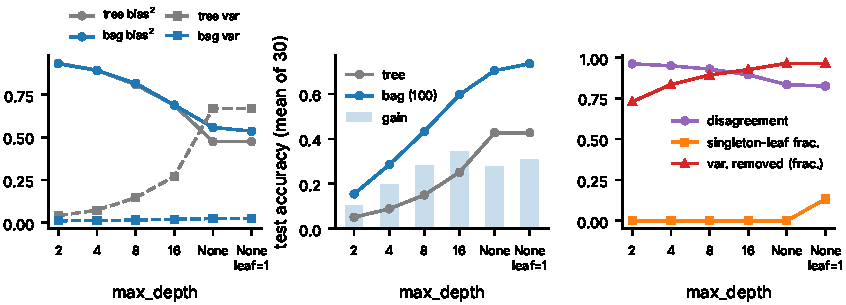
\includegraphics[width=0.92\linewidth]{../figures/q3_depth.pdf}
\caption{Depth study (means over 30 resampled training sets). Left: bias$^2$
(solid) and variance (dashed) for the single tree and 100-tree bagging. Middle:
mean test accuracy and bagging's gain. Right: disagreement among the bagged
trees, fraction of singleton leaves in the bagged trees, and fraction of the
tree's variance removed by bagging.}
\label{fig:q3}
\end{figure*}

\subsection{(c) Is the deepest tree where bagging helps most?}
No. The gain is largest at depth 16 (+34.6 points), smaller for unbounded trees
(+27.8 and +30.8) and smallest for shallow ones (+10.4 at depth 2). With a
standard error of about 1.1 points, the gap is real.

At depth 16 a tree has about 18 leaves of 13 images, so it can name only 18
people, and which 18 depends strongly on the sample. The bagged trees disagree
a lot (0.894) and together cover everyone, so the removed variance (0.25) turns
straight into accuracy. Unbounded trees lose even more variance (0.65), but they
already have one leaf per person, agree more (0.834), and what is left looks
like systematic confusion, such as identities 25 and 37 in Q1(d), which
averaging cannot fix. Shallow trees disagree the most (0.95--0.96) but bias
dominates ($\ge0.89$): every tree misses most people, so there is little to
average. The gain peaks where bias is moderate and disagreement is still high,
which here is depth 16.

\subsection{(d) Summary table}
\begin{table}[h]
\centering\small
\begin{tabular}{lcccc}
\toprule
& clean acc & masked acc & bias$^2$ & variance\\
\midrule
Tree (None, leaf 4)   & 55.0 & 23.8 & .475 & .670\\
Bagging (200)         & \textbf{81.3} & \textbf{67.5} & .558 & .020\\
Boosting (d4, 100)    & 46.3 & 35.0 & .885 & \textbf{.018}\\
\bottomrule
\end{tabular}
\caption{Frozen models: clean and masked test accuracy (\%), with bias$^2$ and
variance from the 30 refits. On the masked set the refit bias$^2$/variance are
tree .794/.737, bagging .715/.021, boosting .895/.019.}
\label{tab:final}
\end{table}

\Cref{tab:final} brings the main numbers together.

\textbf{Most stable:} bagging. Its variance is a thirtieth of the tree's and its
accuracy varies least across refits ($\pm4.3$); the flat disagreement and margin
curves in \cref{fig:bagc} say the same. Boosting's variance is slightly lower,
but only because its $q$ vectors are very flat (largest entry about 0.11). Its
predictions actually swing the most ($\pm7.3$, from 17.5\% to 46.3\%).

\textbf{Most sensitive to the mask:} the single tree. It loses 31.3 points,
sends most masked faces to one leaf, and over the refits scores
$23.5\pm9.3$ on masked faces. Bagging loses 13.8 points and stays the best
masked model; boosting loses 11.3 but started low and falls into a sink
class.

\textbf{Is lowest variance best?} No. Boosting has the lowest variance and the
worst accuracy because its bias is the highest. Accuracy follows the total
bias$^2$+variance (bagging 0.58, boosting 0.90, tree 1.15) much better than
variance alone. Lower variance helps only when bias stays similar, which is
exactly what bagging does for the tree.

{\small
\begin{thebibliography}{9}\setlength{\itemsep}{0pt}
\bibitem{breiman96} L.~Breiman. Bagging predictors. \emph{Machine Learning}, 24(2):123--140, 1996.
\bibitem{zhu09} J.~Zhu, H.~Zou, S.~Rosset, T.~Hastie. Multi-class AdaBoost. \emph{Statistics and Its Interface}, 2(3):349--360, 2009.
\bibitem{freund97} Y.~Freund, R.~E.~Schapire. A decision-theoretic generalization of on-line learning and an application to boosting. \emph{JCSS}, 55(1):119--139, 1997.
\bibitem{samaria94} F.~Samaria, A.~Harter. Parameterisation of a stochastic model for human face identification. \emph{IEEE WACV}, 1994.
\bibitem{kohavi96} R.~Kohavi, D.~Wolpert. Bias plus variance decomposition for zero-one loss functions. \emph{ICML}, 1996.
\end{thebibliography}}
\end{document}
